\chapter{Background}
\label{chp:background} 

This thesis describes the setup and usage of an End-to-End \gls{iot} system. In order for this to be set up by others later to perform reproducible tests, a detailed description of components, sensors and protocols used is needed. This chapter will go through the background information of the devices, technologies and protocols used, and why these where chosen over other alternatives. 

%\section{Internet of Things} % Tjae

%Comment: Read Future Internet: The Internet of Things from 2010.  \cite{gubbi2013internet}

%Comment: Read http://ac.els-cdn.com/S1570870512000674/1-s2.0-S1570870512000674-main.pdf?_tid=6f15526e-eae8-11e5-addc-00000aab0f6b&acdnat=1458072152_0740a71f559cd8ae1ebd0ce4a687e122

%M2M and "M2T" ("Machine to Thing-communication"). Classification of a thing? \cite{tan2010future}. 

%\section{Challenges}


\section{Bluetooth Low Energy}

%Read this:

\gls{ble}, also known as \textit{Bluetooth Smart}, is a wireless technology for short range communication developed by the Bluetooth Special Interest Group. The idea was to create a low energy single-hop network solution for \glspl{pan}. A major advantage of this solution is that Bluetooth 4.0 already is a well established technology in cell phones, laptops and several other devices. This means that few changes needs to be made to these devices to be able to work with bluetooth smart. Still to this date, a device that only implements \gls{ble} is not able to communicate with a device that only implements classic Bluetooth \cite{gomez2012overview}.
The 6LoWPAN Working Group has recognized the importance if \gls{ble} in \gls{iot} \cite{hui2008extending} \todo{Denne linken snakker om 6lowpan, flytte til etter jeg har presentert 6LoWPAN?}.

\begin{figure}[ht]
    \centering
    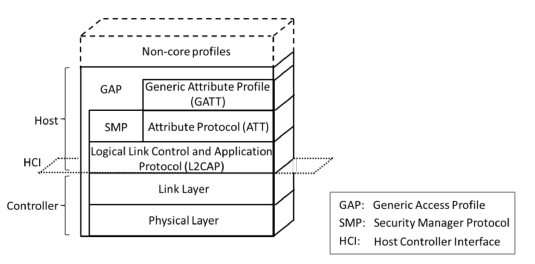
\includegraphics[scale=0.7]{BLEprotocolStack.png}    
    \caption{BLE protocol stack}
    \label{fig:BLEprotocolStack}
\end{figure}

The protocol stack of \gls{ble} has two main parts, the controller and the host, as shown in \ref{fig:BLEprotocolStack}. In the system presented in this thesis this represents the Raspberry Pi as the controller (master) and Nordic nRF52 as the host (slave). The communication between these is done through the standard \gls{hci}. All slaves are in sleep mode by default, and are woken up by the master when communication is needed. Links are being identified by a randomly generated 32-bit code, and the \gls{ism} band used is 2,4 GHz \cite{gomez2012overview}. Other protocols used include \gls{l2cap} used to multiplex data between higher protocol layers, and the segmentation and reassembly of packets. From here packets are being passed to the \gls{hci}, which is the interface used to communicate between the two \gls{ble} devices. This is being used in conjunction with \gls{acl}, which is used to create the \gls{tdma} scheme used to transfer packets over the network link, as well as controlling uptime of the end nodes, as this link is set to disconnect automatically after a given time period if there is no activity on the link. 



\begin{figure}[ht]
    \centering
    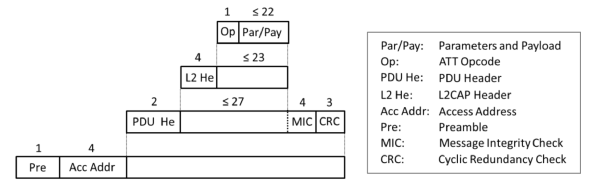
\includegraphics[scale=0.7]{BLEdataUnitStructure.png}    
    \caption{BLE Data Unit Structure}
    \label{fig:BLEdataUnitStructure}
\end{figure}

Figure \ref{fig:BLEdataUnitStructure} shows the data unit structure in \gls{ble}, meaning the different fields that can be used in a packet. The header fields of 4 \gls{byte} of access addresses and \gls{l2cap} will be central topics of discussion later in this thesis. The figure shows that the maximal packet size in a network like this is 31 bytes per packet.  In the case of the network presented here, when the \gls{ble} slave has been connected to a master, it stops searching for other masters, and it is not possible to connect to several masters. This means that we are only able to create a \textit{star network}, not a \textit{mesh network}. This could possibly be an idea for improvement later. Other than this, \gls{ble} seems like a very good alternative in this project. 

%Check out: Mikhail Galeev - BLE

\section{6LoWPAN}

%To identify sensors and devices in low energy sensor and device networks, a new protocol was needed. 

\gls{6lowpan} is a defined protocol for using \gls{ipv6} in low energy networks, to identify sensors and devices, as defined in the IEEE 802.15.4. 

To use the Internet Protocol in low energy networks in addition to standard networks was proposed by Geoff Mulligan and the 6LoWPAN Working Group. In \cite{mulligan20076lowpan}, the advantage of \gls{6lowpan} is explained as 

\textit{Utilizing IP  in these networks and pushing it to the very edge of the network devices flattens the naming and addressing hierarchy and  thereby  simplifies  the  connectivity  model. This obviates the need  for  complex  gateways  that,  in  the  past,  were  necessary  to translate   between   proprietary   protocols   and   standard   Internet Protocols and instead can be replaced with much simpler bridges and  routers,  both  of  which  are  well  understood, well  developed and  widely  available  technologies \cite{mulligan20076lowpan}.}


\gls{6lowpan} was developed to be used in small sensor networks, and implementations can fit into 32Kb flash memory parts. The \gls{mtu} is given to be 1280 byte, and it also uses an impressive header comparison mechanism that allows the transmission of \gls{ipv6} packets in 4 bytes, much less than the standard \gls{ipv6} 40 bytes. This is done by using stacked headers, same as in the \gls{ipv6} model, rather than defining a specific header as for \gls{ipv4}. The device can send only the required part of the stack header, and does not need to include header fields for networking and fragmentation \cite{hui2008extending}. The maximum packet size of the physical layer is set to be 127 bytes, far below the limit of 1280 byte \cite{kushalnagar2007transmission}. It is expected that other layers will produce packets of the desired size to fit the system. In the system presented in this thesis by the example code on the nRF52 is the side set to 270 bytes for every packet, as will be shown later in the thesis. 


%The \gls{6lowpan} architecture was developed to allow \gls{ipv6} packets to be sent over low energy networks.  

\section{Raspberry Pi}

Developed by Newark Element 14 \cite{newark}, the Raspberry Pi has become a central tool for many people wanting to get started using small computers. The device has been known as a single-board computer the size of a credit card specially designed for small network projects and to be used as an educational tool used all the way from elementary schools to here at \gls{ntnu}. This was therefore a natural device to use as a starting point in this system as well. 

\begin{figure}[ht]
    \centering
    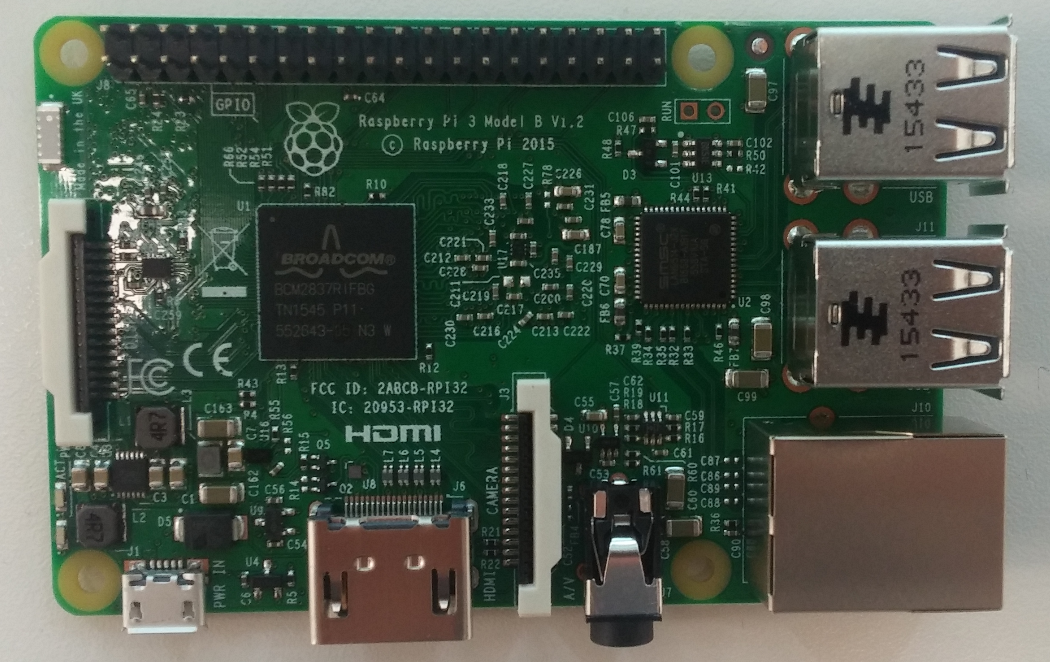
\includegraphics[scale=0.35]{pi3.png}    
    \caption{Raspberry Pi 3}
    \label{fig:piPicture}
\end{figure}

The Raspberry Pi model 3 was released in February 2016, just in time to become a part of the system set up in this project. This includes a \gls{cpu} speed of 1,2 GHz and 1 GB of \gls{ram}. This makes it approximately 12 times faster than the first Raspberry Pi. Both Bluetooth and WiFi is included, and it was quite easy to set up, given that the right Unix kernel has been used in the \gls{os} of the Pi. Along with the Raspberry Pi, we needed a good and stable operating system with a kernel that supported the \gls{6lowpan} architecture. For this, Ubuntu Mate version 15.10 with kernel version 4.15 was chosen, and used on the Raspberry Pi. As other versions of Ubuntu this is Unix based, and has a complete \gls{gui} of a full \gls{os}. The set up of this will be explained in chapter \ref{chp:architecture}.1. 

\section{nRF52}

The most central device of this network is the microcontroller used as end-nodes, the nRF52 developed by Nordic Semiconductor with the \gls{iot} development kit. This is presented as a family of highly flexible, multi-protocol system on chip devices. 



\begin{figure}[ht]
    \centering
    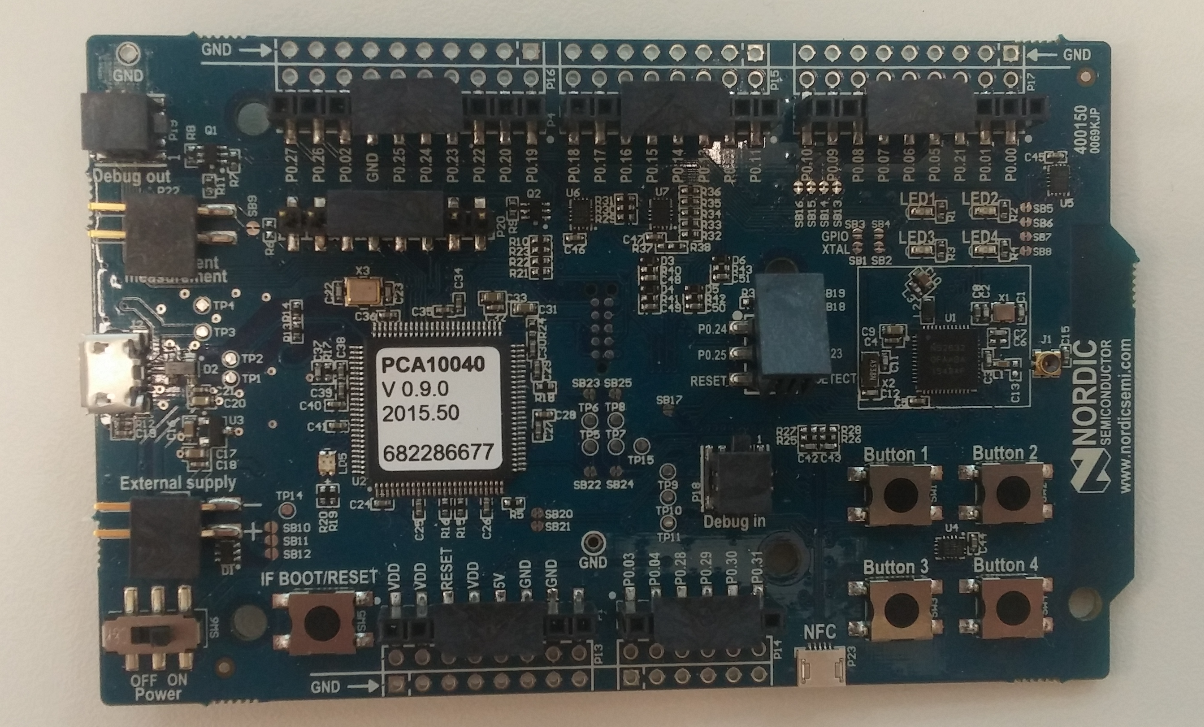
\includegraphics[scale=0.32]{nrf52.png}    
    \caption{Nordic Semiconductor nRF52  }
    \label{fig:nrf52picture}
\end{figure}

\cite{nrf52Nordic}

This device has been advertised as a powerful multiprotocol single chip solution, with both a 32-bit ARM processor, a 512kB flash and 64kB og flash memory. The building blocks of the chip in its entirety is shown in \ref{fig:nrf52chipDetail}. The key features mentioned by Nordic themselves are: 

\begin{itemize}
	\item Multi-protocol 2.4GHz radio
	\item 32-bit ARM Cortex M4F processor
	\item 512kB flash + 64kB RAM
	\item Software stacks available as downloads
	\item Application development independent from protocol stack
	\item On-air compatible with nRF51, nRF24AP and nRF24L Series
	\item Programmable output power from +4dBm to -20dBm
	\item RSSI
	\item RAM mapped FIFOs using EasyDMA
	\item Dynamic on air payload length up to 256 Bytes
	\item Flexible and configurable 32 pin GPIO
	\item Programmable Peripheral Interface – PPI
	\item Simple ON/OFF global power modes
	\item Full set of digital interfaces including: SPI/2-wire/UART/PDM/
	\item I2S, all with EasyDMA
	\item 12-bit/200KSPS ADC
	\item 128-bit AES ECB/CCM/AAR co-processor
	\item Quadrature demodulator
	\item Low cost external crystal 32MHz ± 40ppm for Bluetooth, 	
± 50ppm for ANT
	\item Low power 32MHz crystal and RC oscillators
	\item Ultra low-power 32kHz crystal and RC oscillators
	\item Wide supply voltage range (1.7 V to 3.6 V)
	\item On-chip DC/DC buck converter
	\item Individual power management for all peripherals
	\item Package options: 48-pin 6x6 QFN/WL-CSP
\end{itemize}


In other words much more different options than will be used in this system. The important part here is the processing power, the PPI, the \gls{i2c} bus and the bluetooth antenna. That these things combined can run on only a 3V CR2032 battery is unbelivable. 

%\cite{nrf52Nordic2}


\begin{figure}[ht]
    \centering
    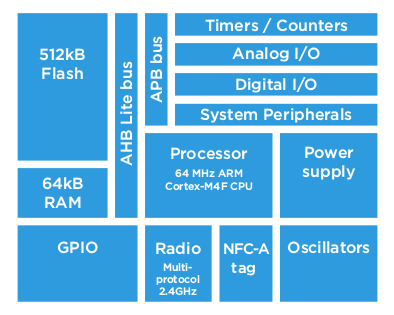
\includegraphics[scale=0.6]{nrf52Detailed.png}    
    \caption{Nordic Semiconductor nRF52 chip in detail }
    \label{fig:nrf52chipDetail}
\end{figure} 

Figure \ref{fig:nrf52chipDetail} shows how the different parts are placed on the chip. 

% https://www.nordicsemi.com/Products/nRF52-Series-SoC
In order to run compiled code on the nRF52, a preprogrammed \textit{Soft device} has to be loaded onto the chip. There are several versions that can be downloaded from http://www.nordicsemi.com. 




\section{Adafruit ADXL345 Accelerometer}

In order to do collect data, a sensor needed to be connected to the Nordic Semiconductor nRF52. The main thought behind the thesis was to measure vibrations, and a good accelerometer was needed. The Adafruit ADXL345 accelerometer was chosen for several reasons. 

\begin{itemize}
  \item It is the same accelerometer built in on the Zolertia Z1 microcontroller
  \item It can measure acceleration in all three axes, X, Y and Z.
  \item It sends digital data right away. This means there is no need to use computational power to calculate digital values as needed if the data was captured by an analog accelerometer. 
  \item It supports both \gls{i2c} and \gls{spi}, which makes it easy to connect to the nRF52. 
\end{itemize}


\begin{figure}[ht]
    \centering
    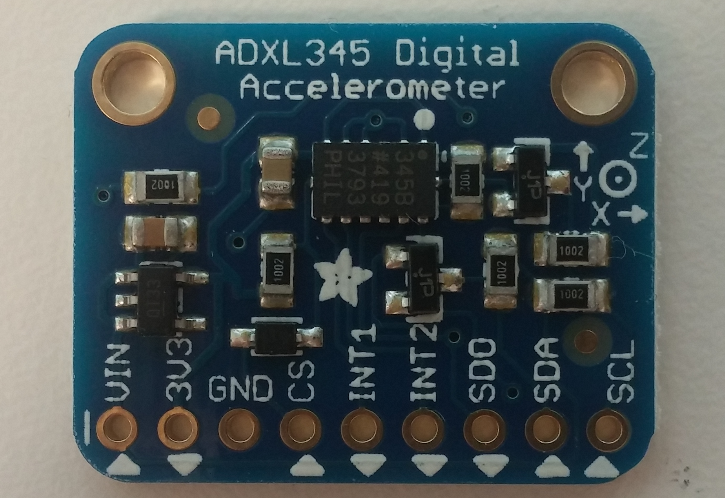
\includegraphics[scale=0.32]{ADXL345.png}    \caption{ADXL345 Accelerometer}
    \label{fig:adxl345}
\end{figure}

\newpage

\section{Transport protocols}

In order to transfer data from the end nodes to the central points of the network, either for analysing or already analysed data, a fast, efficient and stable transport protocol has to be used. This is a central aspect in this network, because the limitations of sending rate is thought to be one of the main limitations, either in the form of limits of data at once or number ofsendings pr second. The protocol needs to be stable and energy efficient and work with both \gls{ble} and \gls{6lowpan}. Luckily, Nordic Semiconductor provides example code and examples on how to get started with this.

\subsection{\gls{coap}}

%The \\ protocol is described in the documentation as follows: 

\gls{coap} is a transport protocol designed to be used in constrained networks for \gls{m2m} communication. It is \gls{udp} based, and works good in low-power and lossy networks. It can be used with microcontrollers, and with \gls{ipv6} and \gls{6lowpan}. Both GET and PUSH functionality can be used, as well as \textit{observable} GET. This means that a server can "subscribe" to end notes in the network, and get updates either after a given timespan or when changes have been made. This therefore looked like a promising protocol to use, and was chosen as the main transport protocol to test in the network \cite{shelby2014constrained}.

The main technical features described in \gls{coap} is as follows: 

\begin{itemize}
	\item Web protocol fulfilling M2M requirements in constrained
      environments
	\item UDP binding with optional reliability supporting unicast
      and multicast requests.
	\item Asynchronous message exchanges.
	\item Low header overhead and parsing complexity.
	\item URI and Content-type support.
	\item Simple proxy and caching capabilities.
	\item A stateless HTTP mapping, allowing proxies to be built providing
      access to CoAP resources via HTTP in a uniform way or for HTTP
      simple interfaces to be realized alternatively over CoAP.
	\item Security binding to Datagram Transport Layer Security (DTLS).	
\end{itemize}


CoAP has several similarities with working over \gls{http}, with the same client and server roles. The client sends a request, and the server sends a response back. Many of the response codes are also very similar, with \textit{404: Not found} as the best known. When \gls{m2m} communication is used, both participants sometimes needs to be both client and server, and the \gls {coap} protocol handles this with a two-layer approach. \todo{make figure of CoAP Layering}. There are four different main messages defined in CoAP, being described as follows: 

   Confirmable
	  \textit{Some messages require an acknowledgement.  These messages are
      called "Confirmable".  When no packets are lost, each Confirmable
      message elicits exactly one return message of type Acknowledgement
      or type Reset.}

   Non-confirmable Message
      Some other messages do not require an acknowledgement.  This is
      particularly true for messages that are repeated regularly for
      application requirements, such as repeated readings from a sensor.

   Acknowledgement Message
      An Acknowledgement message acknowledges that a specific
      Confirmable message arrived.  By itself, an Acknowledgement
      message does not indicate success or failure of any request
      encapsulated in the Confirmable message, but the Acknowledgement
      message may also carry a Piggybacked Response (see below).
      
Other messages used is \textit{GET, PUT, POST and DELETE}, to get or change data stored on the server. 
      

\begin{figure}[ht]
    \centering
    \includegraphics[scale=0.5]{seqDiagramCoAP.png}    
    \caption{Sequence diagram CoAP}
    \label{fig:seqDiagramCoAP}
\end{figure}

\begin{figure}[ht]
    \centering
    \includegraphics[scale=0.6]{CONclientserver.png}    
    \caption{CON CoAP client server sequence diagram}
    \label{fig:CONclientserver}
\end{figure}


\begin{figure}[ht]
    \centering
    \includegraphics[scale=0.6]{NONOackSeqDiagram.png}    
    \caption{NON CoAP client server sequence diagram}
    \label{fig:NONOackSeqDiagram}
\end{figure}


\begin{figure}[ht]
    \centering
    \includegraphics[scale=0.6]{CoAPMessageFormat.png}    
    \caption{CoAP message format}
    \label{fig:CoAPMessageFormat}
\end{figure}



\begin{figure}[ht]
    \centering
    \includegraphics[scale=0.6]{CoAPUsageOfMessageTypes.png}    
    \caption{CoAP usage of message types}
    \label{fig:CoAPUsageOfMessageTypes}
\end{figure}



\subsection{\gls{mqtt}}

Another transport protocol that could be used in such a network of microcontrollers is \gls{mqtt}. This is  known as a publish-subscribe based on \gls{tcp}, using a \gls{mqtt} broker. \gls{ntnu} does have a broker that is possible to use, or a broker can be rented from several other places. Here a 

\cite{hunkeler2008mqtt}

\subsection{\gls{radvd}}


\section{Software tools}

As \gls{ide}, the \textit{KEIL Vision} was used, as recommended by Nordic Semiconductor (where?), for writing C programming. For other programming languages (for instance Python 3.4, HTML, CSS, JavaScript, Flask and AJAX) \textit{Sublime Text 2} for Windows and Linux was used, as well as \textit{Pluma} for Ubuntu Mate on the Raspberry Pi. 

\subsection{Other}

Wireshark, Firefox, GitHub


\subsection{Abbreviations used in the rest of this thesis}




